% Created 2024-08-24 Sat 19:57
% Intended LaTeX compiler: lualatex
\documentclass{beamer}
\usetheme{default}
\author{fabio}
\date{\today}
\title{}
\hypersetup{
 pdfauthor={fabio},
 pdftitle={},
 pdfkeywords={},
 pdfsubject={},
 pdfcreator={Emacs 29.4 (Org mode 9.6.15)}, 
 pdflang={English}}
\begin{document}

\begin{frame}{Sumário}
\tableofcontents
\end{frame}

\begin{frame}[label={sec:org5143cec}]{Reações Orgânicas}
\begin{block}{Reações Orgânicas}
Reações orgânicas são formas de transformação de moléculas orgânicas em outras moléculas orgânicas. São tipos de reações orgânicas:
\begin{itemize}
\item Reações de adição
\item Substituição
\item Oxidação
\item Redução
\item Eliminação.
\end{itemize}
\end{block}
\end{frame}

\begin{frame}[label={sec:orgefcf320}]{Alcanos}
\begin{block}{Alcanos}
\begin{itemize}
\item Carbono e hidrogênio têm eletronegatividades bem semelhantes, logo, a ligação C - H é basicamente apolar.
\item Conseqüentemente, compostos contendo ligações C - C e C - H são estáveis e apresentam uma tendência muito baixa para reagir com outras substâncias.
\item A adição de grupos funcionais (por exemplo, C-O-H) introduz reatividade às moléculas orgânicas.
\item Suas reações envolvem a formação de radicais, formados em altas temperaturas ou na presença de radiação UV.
\end{itemize}
\end{block}

\begin{block}{Formação de Radicais}
\alert{Radicais:} espécies químicas que apresentam um elétron desemparelhado.

\begin{reaction}
	R3C-X -> R3 "\chlewis{0.}{C}"  +  "\chlewis{180.}{X}"
\end{reaction}


\begin{bclogo}[couleur=blue!30 , arrondi=0.1 , logo=\bcplume , epBarre=3.5]{Estabilidade do Radicais Alquila}
\begin{center}	
\chemfig{R-\charge{0=\.}{C}([:90]-R)([:-90]-R)} \qquad > \qquad \chemfig{R-\charge{0=\.}{C}([:90]-H)([:-90]-R)} \qquad > \qquad \chemfig{H-\charge{0=\.}{C}([:90]-H)([:-90]-H)}
\end{center}
\end{bclogo}
\end{block}

\begin{block}{Halogenação}
\begin{itemize}
\item Sob condições adequadas sofrem reação de substituição com halogênios.
\item A substituição de um \alert{H} por um halogênio é denominada \alert{halogenação}.
\end{itemize}



\begin{bclogo}[couleur=blue!30 , arrondi=0.1 , logo=\bcplume , epBarre=3.5]{Cloração do Metano}
\begin{reaction*}
CH4 + C$\ell$2(excesso) ->[$\Delta$ ou][h$\nu$] CH3C$\ell$ + CH2C$\ell$2 + CHC$\ell$3 + CC$\ell$4 + HC$\ell$
\end{reaction*}	 
\end{bclogo}
\end{block}


\begin{block}{}
\begin{bclogo}[couleur=blue!30 , arrondi=0.1 , logo=\bcplume , epBarre=3.5]{Mecanismo de cloração do Metano}

  \begin{empheq}[left=\text{Inicia\c{c}\~{a}o}\quad\; \empheqlbrace]{flalign} 
	\ch{C$\ell$2 -> 2 "\chlewis{0.}{C$\ell$}"} & \qquad \qquad \qquad \quad \quad   \enthalpy{-242.7}
	\end{empheq}
	
	%%%% Reac2
 \begin{empheq}[left=\text{Propaga\c{c}\~{a}o}\; \empheqlbrace]{flalign}
	\ch{"\chlewis{0.}{C$\ell$}" + CH4 -> "\chlewis{180.}{C}" H3 + HC$\ell$} & \quad \qquad \enthalpy{-3.4}\\
	\ch{"\chlewis{180.}{C}" H3{} + {} C$\ell$2 -> CH3C$\ell$ + "\chlewis{180.}{C}" $\ell$} & \quad \qquad	\enthalpy{-106.7}
\end{empheq}

%%% R3

 \begin{empheq}[left=\text{T\'ermino}\;\quad \empheqlbrace]{flalign}
\ch{"\chlewis{0.}{C$\ell$}" {} + {}  "\chlewis{0.}{C$\ell$}" {} -> C$\ell$2} & \qquad \qquad \enthalpy{-242.7} \\ 
\ch{"\chlewis{0.}{C$\ell$}" {} + {}  "\chlewis{180.}{C}" H3{}  -> CH3C$\ell$} & \qquad \qquad \enthalpy{-349.4}\\
\ch{"\chlewis{180.}{C}" H3{} + "\chlewis{180.}{C}" H3{} -> CH3CH3} & \qquad \qquad \enthalpy{-368.2}
\end{empheq}
\end{bclogo}
\end{block}
\begin{block}{}
\begin{itemize}
\item Todos os outros alcanos reagem com os \alert{halogênios} da mesma maneira que o metano.
\item Quanto maior o número de carbonos, maior será o número de possíveis compostos mono e polialogenados formados.
\end{itemize}


\begin{bclogo}[couleur=blue!30 , arrondi=0.1 , logo=\bcplume , epBarre=3.5]{Mecanismo de cloração do metilpropano}
\schemestart[,1.0]
\chemfig{CH_3-C([:90]-CH_3)([:-90]-H)-CH_3}
\arrow(.mid east--.mid west)
\chemname{\chemfig{CH_3-C([:90]-CH_3)([:-90]-H)-CH_3}}{> 99\%} \quad +  \quad \chemname{\chemfig{CH_3-CH([:90]-CH_3)-CH_2-Br}}{Traços}
\schemestop
\end{bclogo}
\end{block}



\begin{block}{Oxidação}
Os \alert{alcanos} e outros \alert{hidrocarbonetos} queimam na presença \ch{O2}, sendo tal reação de oxidação denominada
\alert{combustão}.


\begin{bclogo}[couleur=blue!30 , arrondi=0.1 , logo=\bcplume , epBarre=3.5]{Mecanismo de combustão dos alcanos}


\begin{align*}
\ch{C_nH_{2n+2}} \quad + \quad  \frac{3n+1}{2}\ch{O2 -> n CO2}\quad +\quad (n+1)\ch{H2O} & \qquad \quad \enthalpy*[unit=\kilo\joule\per\gram]{\approx 55} \approx 55 \unit{\kilo\joule\per\gram}\\ & \hspace{1cm} \mathrm{de~hidrocarboneto} \\ \\
\ch{CH4\gas{} \quad{} + \quad{} 2 O2\gas{} -> CO2\gas{} \qquad{} + \quad{} 2 H2O\lqd{}} & \quad \quad \enthalpy{-891.2}\\ \\
	\ch{2 C4H10\gas{} \quad{} + \qquad{} 13 O2\gas{} -> 8 CO2\gas{} \quad{} + \quad{} 2 H2O\lqd{}} & \quad \quad \enthalpy{-2878.6}    
\end{align*}
\end{bclogo}
\end{block}


\begin{block}{Reação de pirólise}
\begin{itemize}
\item \alert{Pirólise} é um tipo de reação de decomposição ou análise, em que uma substância é decomposta em outras, pela ação do calor do fogo.
\end{itemize}



\begin{bclogo}[couleur=blue!30 , arrondi=0.1 , logo=\bcplume , epBarre=3.5]{Mecanismo de Pirólise}



\begin{figure}
\setchemfig{atom sep=1.6em}
\tiny{	
%\setchemfig{scheme debug=true}
\schemestart[,1.0]
\chemfig{H-C([:90]-H)([:-90]-H)-C([:90]-H)([:-90]-H)-C([:90]-H)([:-90]-H)-C([:90]-H)([:-90]-H)-C([:90]-H)([:-90]-H)-C([:90]-H)([:-90]-H)-C([:90]-H)([:-90]-H)-C([:90]-H)([:-90]-H)-C([:90]-H)([:-90]-H)-C([:90]-H)([:-90]-H)-C([:90]-H)([:-90]-H)-C([:90]-H)([:-90]-H)-C([:90]-H)([:-90]-H)-C([:90]-H)([:-90]-H)-C([:90]-H)([:-90]-H)-C([:90]-H)([:-90]-H)-H} 
\arrow{->[*{0}Aquecimento]}[-90]%(@c1--)[-90]
\chemfig{H-C([:90]-H)([:-90]-H)-C([:90]-H)([:-90]-H)-C([:90]-H)([:-90]-H)-C([:90]-H)([:-90]-H)-C([:90]-H)([:-90]-H)-C([:90]-H)([:-90]-H)-C([:90]-H)([:-90]-H)-\charge{0=\.}{C}@{db,1.3}([:90]-H)([:-90]-H)} \qquad  + \qquad 
\chemfig{\charge{180=\.}{C}([:90]-H)([:-90]-@{atoo,1.5}H)-[@{a2}]C([:90]-H)(-[@{a1}:-90]H)-C([:90]-H)([:-90]-H)-C([:90]-H)([:-90]-H)-C([:90]-H)([:-90]-H)-C([:90]-H)([:-90]-H)-C([:90]-H)([:-90]-H)-C([:90]-H)([:-90]-H)-H}
\arrow(@c2--)[-90]
\chemfig{H-C([:90]-H)([:-90]-H)-C([:90]-H)([:-90]-H)-C([:90]-H)([:-90]-H)-C([:90]-H)([:-90]-H)-C([:90]-H)([:-90]-H)-C([:90]-H)([:-90]-H)-C([:90]-H)([:-90]-H)-C([:90]-H)([:-90]-H)-H} \quad + \quad \chemfig{H-C([:90]-H)=C([:90]-H)-C([:90]-H)([:-90]-H)-C([:90]-H)([:-90]-H)-C([:90]-H)([:-90]-H)-C([:90]-H)([:-90]-H)-C([:90]-H)([:-90]-H)-C([:90]-H)([:-90]-H)-H}
\schemestop 
\chemmove{
\draw[shorten <=2pt, shorten >=2pt](db) ..controls +(down:10mm) and +(150:8mm)..(atoo);
\draw[shorten <=2pt, shorten >=2pt](a1) ..controls +(135:1mm) and +(250:5mm)..(a2);
}}
\caption{Esquema de pirólise do hexadecano, com formação do octano e oct-1-eno.}
\end{figure}
\end{bclogo}
\end{block}


\begin{block}{Reação de isomerização}
\begin{bclogo}[couleur=blue!40 , arrondi=0.1 , logo=\bcplume , epBarre=3.5]{Isomerização dos alcanos}


\setchemfig{atom sep=1.8em}
\begin{figure}
\small{
\centering
\schemestart
\subscheme{%
\chemname{\chemfig{CH_3-CH([:90]-CH_3)-CH_3}}{Isobutano}
\arrow{<<->[\ch{A$\ell$C$\ell$3}][\SI{27}{\degreeCelsius}]}[180,1.2] 
\chemfig{H_3C-CH_2-CH_2-CH_3}
}
\schemestop
\vspace{0.5cm}
\schemestart
\chemfig{CH_3-{(}CH_2{)}_5-CH_3}
\arrow{->} \chemname{\chemfig{CH_3-CH([:90]-CH_3)-CH_2-CH_2-CH_2-CH_3}}{2-metileptano}
\schemestop
}
\caption{Exemplos de reações de isomerização no alcanos}
\end{figure}
\end{bclogo}
\end{block}
\end{frame}


\begin{frame}[label={sec:orgd3ecc3c}]{Alcenos}
\begin{block}{Reação de adição}
\begin{itemize}
\item Os alcenos participam de reações de adição, nas quais os fragmentos da quebra de pequenas moléculas, tais como, \ch{H2}, \ch{C$\ell$2}, \ch{HC$\ell$} e \ch{H2O}, se adicionam aos carbonos que estabeleciam ligação dupla e que após a reação, passam a estabelecer ligação simples.
\end{itemize}



\begin{bclogo}[couleur=blue!40 , arrondi=0.1 , logo=\bcplume , epBarre=3.5]{Isomerização dos alcanos}
\begin{center}
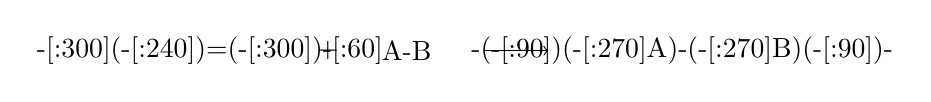
\begin{tikzpicture}
	\node[draw=none] at (0,0) {\chemfig{-[:300](-[:240])=(-[:300])-[:60]}};
	\node[draw=none] at (1.5,0) {+};
	\node[draw=none] at (2.5,0) {A-B};
	\draw[->] (3.5,0)--(4.3,0);
	\node[draw=none] at (6,0) {\chemfig{-(-[:90])(-[:270]A)-(-[:270]B)(-[:90])-}};
\end{tikzpicture}
\end{center}

Onde \alert{AB} =  \ch{H2}, HX, \ch{H2O}, \ch{X2}, ROH 
\end{bclogo}
\end{block}


\begin{block}{}
\vspace{-.5cm}
\begin{itemize}
\item O termo \alert{carbocátion} foi sugerido por George A. Olah para designar qualquer espécie catiônica do carbono. Os carbocátions têm deficiência de elétrons, com apenas 6 elétrons na camada de valência e, por causa disto, são ácidos de Lewis.
\end{itemize}

\begin{bclogo}[couleur=blue!40 , arrondi=0.1 , logo=\bcplume , epBarre=3.5]{Formação do carbocátions}
\begin{center}
\schemestart	
	\chemname{\chemfig{R_2-\charge{[extra sep=0pt]45 [anchor=180+\chargeangle]=$\scriptstyle\oplus$}{C}([:90]-R_1)([:-90]-R_3)}}{Terciário} \qquad > \qquad \chemname{\chemfig{R_2-\charge{[extra sep=0pt]45 [anchor=180+\chargeangle]=$\scriptstyle\oplus$}{C}([:90]-R_1)([:-90]-H)}}{Secundário} \qquad > \qquad \chemname{\chemfig{R_1-\charge{[extra sep=0pt]45 [anchor=180+\chargeangle]=$\scriptstyle\oplus$}{C}([:90]-H)([:-90]-H)}}{Primário}\qquad > \qquad \chemname{\chemfig{H-\charge{[extra sep=0pt]45 [anchor=180+\chargeangle]=$\scriptstyle\oplus$}{C}([:90]-H)([:-90]-H)}}{Metil}
	\schemestop
	\chemmove{
	\node[single arrow, draw=black, fill=red8!30, 
	minimum width = 10pt, single arrow head extend=3pt,
	minimum height=10mm, below=1cm of c1,font=\bfseries] {Ordem decrescente de estabilidade dos carbocátions}; % length of arrow
	}
	\end{center}
\end{bclogo}
\end{block}

\begin{block}{Adição de hidrogênio ou higrodenação catalítica}
\begin{itemize}
\item Consiste na reação do alceno com gás \ch{H2}, que é catalisada por níquel (\alert{Ni}), platina (\alert{Pt}) ou paládio (\alert{Pd}).
\item Atuação do catalisador na hidrogenação: adsorve tanto as moléculas de \ch{H2} como do alceno, provocando o enfraquecimento das ligações, tornando a reação mais fácil.
\end{itemize}



\begin{bclogo}[couleur=blue!30 , arrondi=0.1 , logo=\bcplume , epBarre=3.5]{Mecanismo de hidrogenação}

\begin{tikzpicture}[thick,scale=0.8, every node/.style={scale=0.8}]

%\draw[help lines] (0,0) grid (2,2);
\tikzstyle{ground}=[fill,pattern=north east lines,draw=none,minimum width=0.3,minimum height=0.6]
\node (wall1) [ground, minimum width=2cm] {};
\draw (wall1.north west) -- (wall1.north east);
\node[above=0.5cm of wall1]{\ch{H2}};
\node[below=0.3cm of wall1,text width=2cm]{Superfície do catalisador};
\node (seta1) [right=0.5cm of wall1]{\ch{<=>}};
%%% ============= Wall 2
\node (wall2) [right=0.5cm of seta1,ground, minimum width=2cm] {};
\draw (wall2.north west) -- (wall2.north east);
\node (seta2) [right=0.5cm of wall2]{\ch{<=>}};
\node(H1)[] at (3.7,0.85){H};
\node(H2)[] at (4.6,0.85) {H};
\draw(wall2)--(H1);
\draw(wall2)--(H2);
%%%% ================== WALL 3 
\node (wall3) [right=0.5cm of seta2,ground, minimum width=2cm] {};
\draw (wall3.north west) -- (wall3.north east);
\node (seta3) [right=0.5cm of wall3]{\ch{->}};
\node(H3)[] at (8.1,0.85){H};
\node(H4)[] at (8.6,0.85){H};
\node(et)[] at (9.3,1.7) {\chemfig[atom style={scale=.7}]{H-[:110]C(-[:55]H)=[:180]C(-[:120]H)-[:240]H}};
\draw(8.1,0)--(H3);
\draw(8.6,0)--(H4);
\draw[dashed] (9.3,0)--(9.3,1.7);
 
 
 %%%%% ================ WALL 4
\node (wall4) [right=0.5cm of seta3,ground, minimum width=2cm] {};
\draw (wall4.north west) -- (wall4.north east);
\node(etano)[above=.5cm of wall4] {\chemfig[atom style={scale=.7}]{H-[:110]C(-[:55]H)(-[:357.5]H)-[:180]C(-[:120]H)(-[:240]H)-[:180]H}};
\end{tikzpicture}
\end{bclogo}
\end{block}

\begin{block}{}
\begin{itemize}
\item Uma aplicação industrial da hidrogenação catalítica é na fabricação de margarinas a partir de óleos vegetais.
\item Óleos Vegetais: misturas de ésteres do glicerol com ácidos graxos. Tais ésteres são denominados \alert{triacilglicerídeos}.
\end{itemize}


\begin{bclogo}[couleur=blue!30 , arrondi=0.1 , logo=\bcplume , epBarre=3.5]{Exemplo de triacilglicerídeo}
\definesubmol{r1}{{[}CH_2{]}_7CH=CHCH_2CH=CHCH_2CH=CHCH_2CH_3}
\definesubmol{r2}{{[}CH_2{]}_7CH=CHCH_2CH=CH{[}CH_2{]}_4CH_3}
\definesubmol{r3}{{[}CH_2{]}_7CH=CH{[}CH_2{]}_7CH_3}
\chemfig[atom sep=2em]{H-C(-[2,2]C(-[4]H_2)-O-C(=[2]O)-!{r1})(-[6,2]C(-[4]H_2)-O-C(=[2]O)-!{r3})-O-C(=[2]O)-!{r2}}
\end{bclogo}
\end{block}


\begin{block}{}
\begin{itemize}
\item Com a hidrogenação parcial das ligações duplas dos triacilglicerídeos, o óleo vegetal é convertido em um material de consistência pastosa denominado \alert{margarina}.

\begin{center}
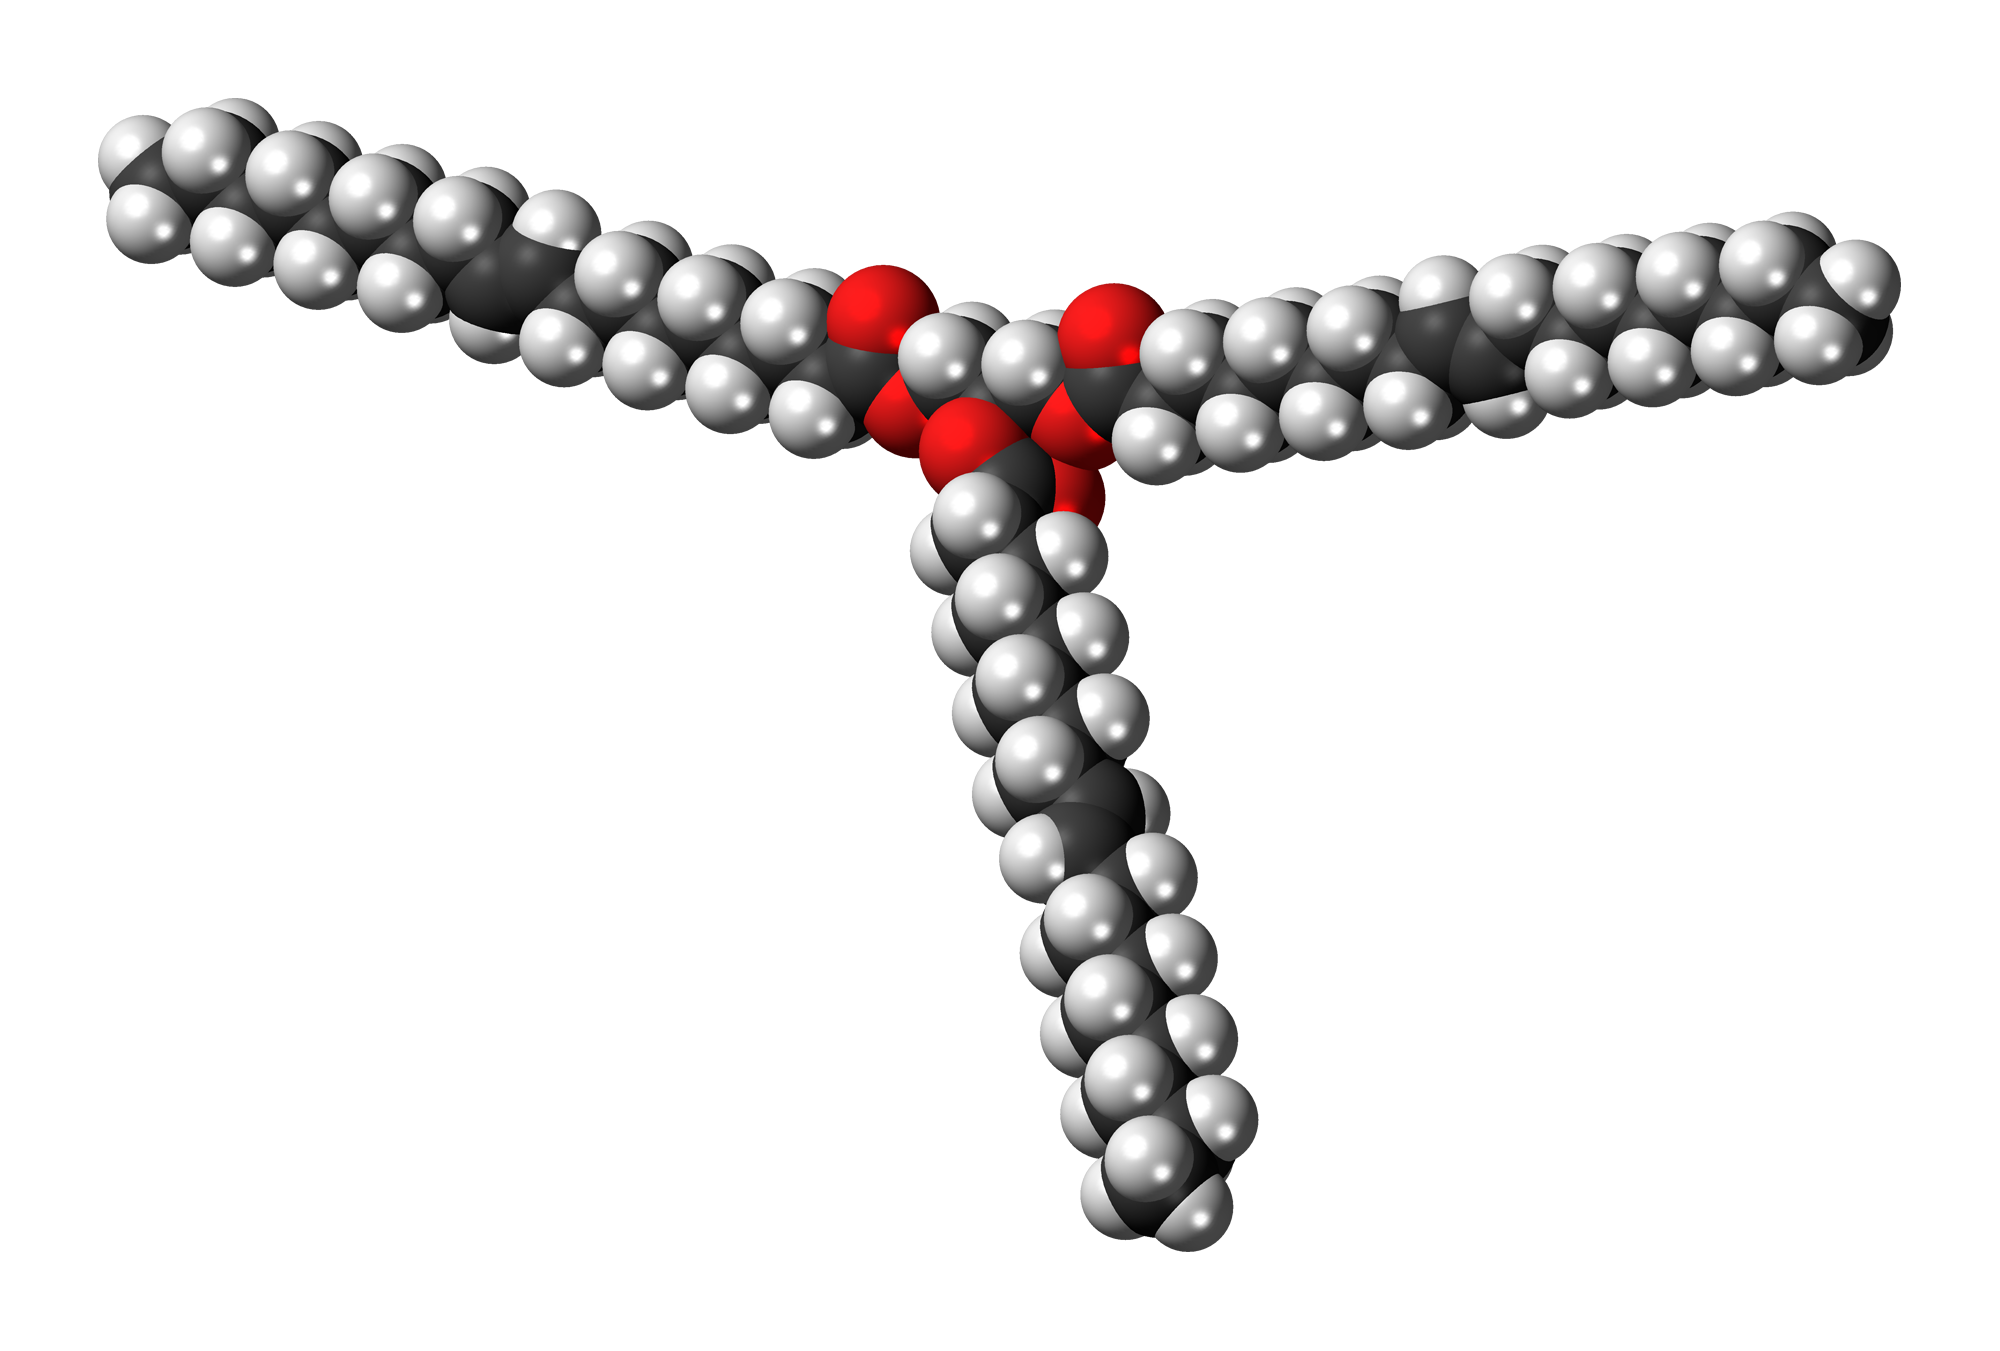
\includegraphics[scale=0.05]{../ReacoesOrganicas/trigli3D.png}
\end{center} \par
\begin{center}
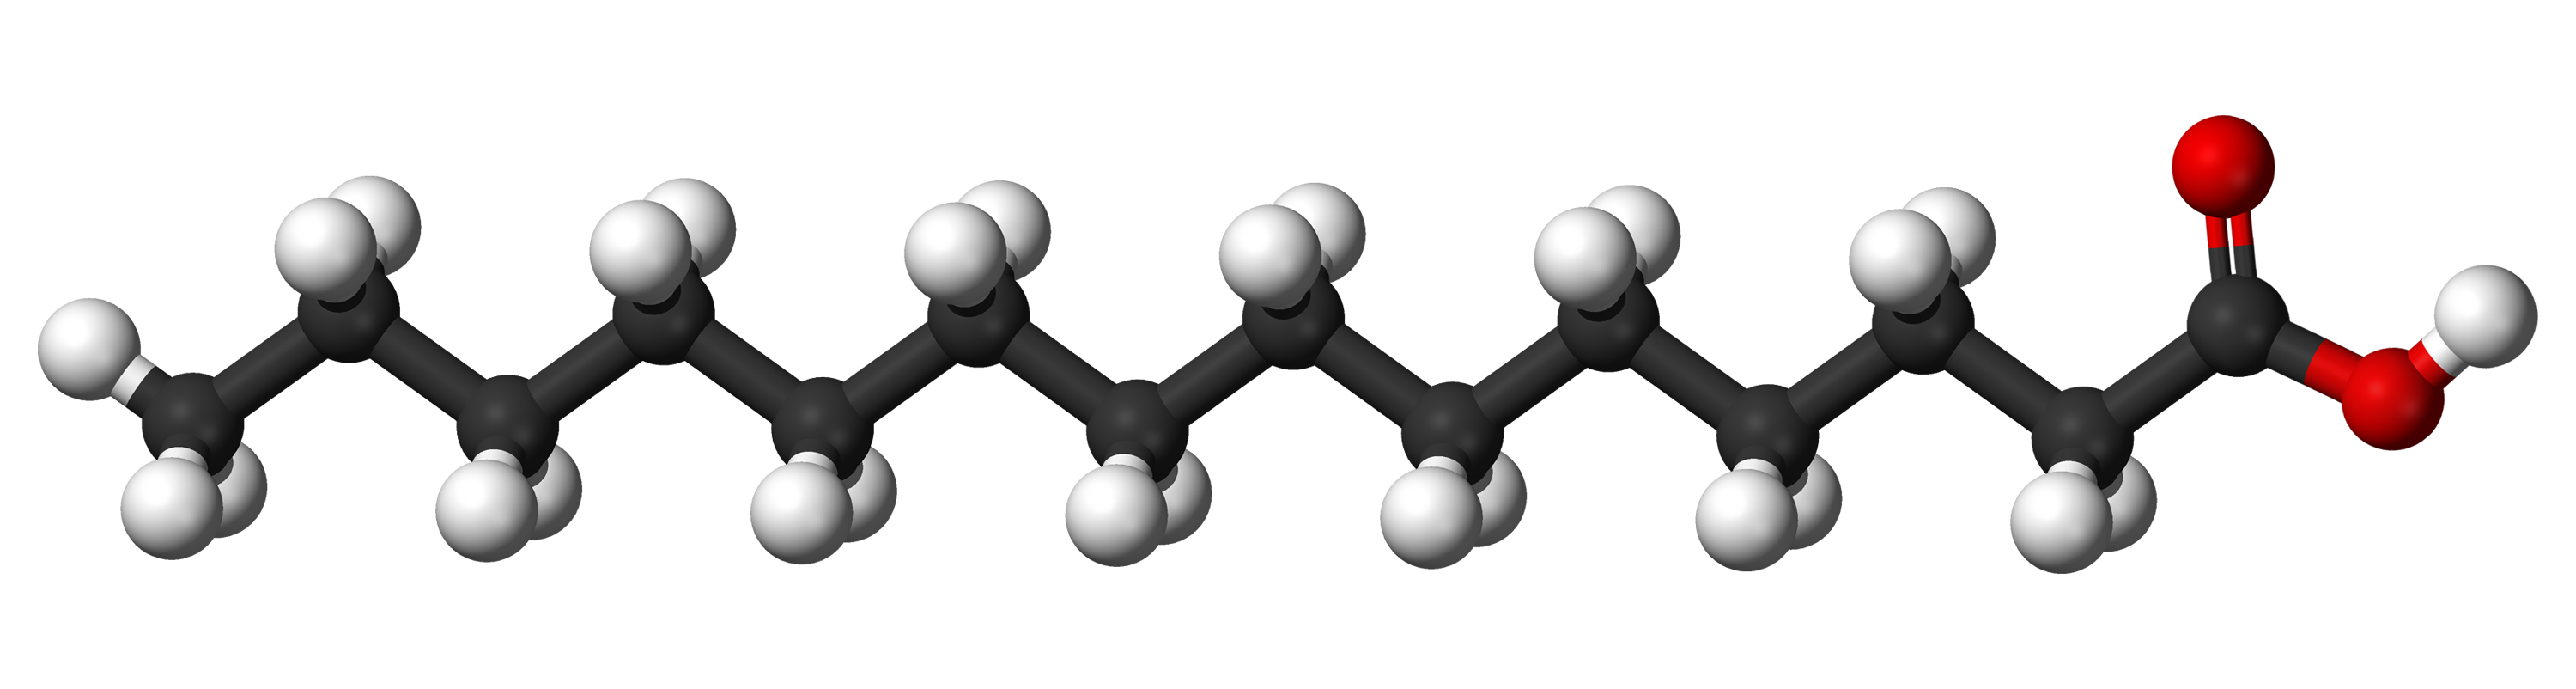
\includegraphics[scale=0.05]{../ReacoesOrganicas/triglimono.png}
\end{center}
\end{itemize}
\end{block}



\begin{block}{Adição de halogênios}
\begin{bclogo}[couleur=blue!30 , arrondi=0.1 , logo=\bcplume , epBarre=3.5]{Adição de halogênios}


\schemestart
%\chemfig{@{a4}H_2C=C@{a3}H_2}
\chemfig{@{a4}C(-[3]H)(-[5]H)=@{a3}C(-[1]H)-[7]H}
\qquad + \qquad 
\chemfig{@{a2}C{\ell}-@{a1}C{\ell}} 
\arrow 
\chemfig{H-C([:90]-C{\ell})([:-90]-H)-C([:90]-C{\ell})([:-90]-H)-H}
\chemmove[-stealth,shorten <=3pt,dash pattern= on 1pt off 1pt,thin]{
\draw[shorten >=2pt](a1) ..controls +(300:7mm) and +(10:5mm)..(a3);
\draw[shorten >=2pt](a2) ..controls +(110:15mm) and +(90:7mm)..(a4);
}
\schemestop
\end{bclogo}
\end{block}

\begin{block}{Adição de haletos de hidrogênio (HX)}
\begin{bclogo}[couleur=blue!30 , arrondi=0.1 , logo=\bcplume , epBarre=3.5]{Adição de haletos}



\schemestart
\chemfig{@{a4}C(-[3]H)(-[5]H)=@{a3}C(-[1]H)-[7]H}
\qquad + \qquad 
\chemfig{@{a2}H-@{a1}C{\ell}} 
\arrow 
\chemfig{H-C([:90]-H)([:-90]-H)-C([:90]-C{\ell})([:-90]-H)-H}
\chemmove[-stealth,shorten <=3pt,dash pattern= on 1pt off 1pt,thin]{
\draw[shorten >=2pt](a1) ..controls +(300:7mm) and +(10:5mm)..(a3);
\draw[shorten >=2pt](a2) ..controls +(110:15mm) and +(90:7mm)..(a4);
}
\schemestop
\end{bclogo}
\end{block}


\begin{block}{Adição de água}
\begin{bclogo}[couleur=blue!30 , arrondi=0.1 , logo=\bcplume , epBarre=3.5]{Adição de água}

\schemestart
\chemfig{@{a4}C(-[3]H)(-[5]H)=@{a3}C(-[1]H)-[7]H}
\qquad + \qquad 
\chemfig{@{a2}H-@{a1}OH} 
\arrow{->[\ch{H^+}]}
\chemfig{H-C([:90]-H)([:-90]-H)-C([:90]-OH)([:-90]-H)-H}
\chemmove[-stealth,shorten <=3pt,dash pattern= on 1pt off 1pt,thin]{
\draw[shorten >=2pt](a1) ..controls +(300:7mm) and +(10:5mm)..(a3);
\draw[shorten >=2pt](a2) ..controls +(110:15mm) and +(90:7mm)..(a4);
}
\schemestop
\end{bclogo}
\end{block}



\begin{block}{Regra de Markovnikov}
\begin{itemize}
\item Ao realizar a adição de HX (X = halogênio) ou \ch{H2O} a um  alceno, se a molécula da substância orgânica não for simétrica em relação à dupla \chemfig{C=C}, poderemos pensar na possibilidade de dois produtos diferentes.
\end{itemize}



\begin{bclogo}[couleur=blue!30 , arrondi=0.1 , logo=\bcplume , epBarre=3.5]{Adição de água}


\begin{center}
\schemestart
\chemfig{H_3C-CH=CH_2} 
	+
	\chemfig{HC{\ell}}
	\arrow(nph.mid east--.south west){->}[30]
	\chemfig{H_3C-CH([:90]-C{\ell})-CH_2([:90]-H)} produto obtido
	\arrow(@nph.mid east--.north west){-/>}[-30]
	\chemfig{H_3C-CH([:90]-H)-CH_2([:90]-C{\ell})} {\color{red} produto não obtido} 
	\schemestop
\end{center}
\end{bclogo}
\end{block}

\begin{block}{}
\begin{columns}
\begin{column}[t]{0.45\columnwidth}
\begin{itemize}
\item Em 1869, o químico Vladimir Markovnikov enunciou uma regra empírica, isto é, baseada em fatos experimentais, conhecida como Regra de Markovnikov
\item \alert{REGRA:} na adição de HX ou \ch{H2O} a uma ligação dupla \alert{C=C}, o átomo de \alert{H} se adiciona preferencialmente ao carbono da dupla que já contém mais hidrogênio, ou seja, o H se adiciona ao carbono mais hidrogenado.
\end{itemize}
\end{column}


\begin{column}[t]{0.45\columnwidth}
\begin{center}
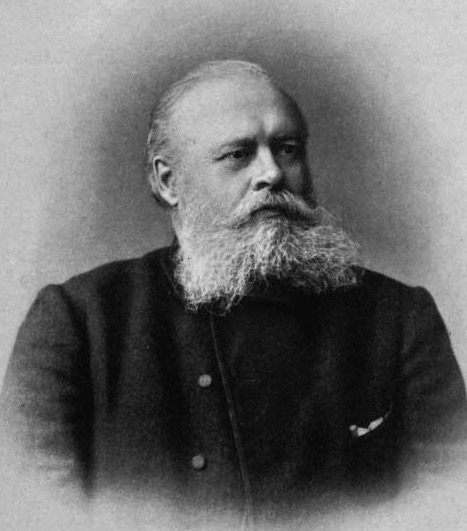
\includegraphics[scale=.5]{./VladimirMarkovnikov.jpg}
\end{center}
\end{column}
\end{columns}
\end{block}



\begin{block}{Exemplos}
\begin{bclogo}[couleur=blue!30 , arrondi=0.1 , logo=\bcplume , epBarre=3.5]{Exemplos da Regra de Markovnikov}
\schemestart
\chemfig{H_3C-CH=CH_2} 
+ 
\chemfig{HC{\ell}}
\arrow(c1.mid east--c2.mid west){->}
\chemfig{H_3C-CH([:90]-C{\ell})-CH_3}
\schemestop
\par \medskip

\schemestart
\chemfig{H_3C-C([:90]-CH_3)=CH_2}
+
\chemfig{HBr}
\arrow(c1.mid east--c2.mid west){->}
\chemfig{H_3C-C([:90]-Br)([:-90]-CH_3)-CH_3}
\schemestop\par \medskip

\schemestart
\chemfig{CH_2=[:180]-[:240]-[:180]-[:120]-[:60]-(-[:300])} + \chemfig{HI}
\arrow{->}
\chemfig{CH_3-[:120](-[:60,,,1]I)-[:240]-[:180]-[:120]-[:60]-(-[:300])}
\schemestop
\end{bclogo}
\end{block}
\end{frame}





\begin{frame}[label={sec:orgfffd2f9}]{Alcinos}
\begin{block}{Reações de Adição}
\begin{itemize}
\item A ligação tripla dos alcinos comporta-se como a dupla dos alcenos, porém pode sofrer uma ou duas adições, dependendo da quantidade do outro reagente.
\end{itemize}

\begin{bclogo}[couleur=blue!30 , arrondi=0.1 , logo=\bcplume , epBarre=3.5]{Adição em Alcinos}

\schemestart
\chemfig{-@{at1}C~@{at2}C-} \quad  \arrow{->[\chemfig{@{a1}\color{red}{A}-\color{blue}{B}@{a2}}]} 
\qquad \chemfig{@{at3}C([:120]-\color{red}{A})([:240]-)=@{at4}C([:60]-\color{blue}{B})([:300]-)} \arrow{->[\chemfig{@{b1}A-B@{b2}}]} \chemfig{-C([:90]-\color{red}{A})([:-90]-A)-C([:90]-\color{blue}{B})([:-90]-B)-}
\schemestop
\chemmove[-stealth,shorten <=3pt]%dash pattern= on 1pt off 1pt,thin]
{
\draw[shorten >=2pt,red](a1) ..controls +(160:7mm) and +(100:15mm)..(at1);
\draw[shorten >=2pt,blue](a2) ..controls +(110:15mm) and +(90:7mm)..(at2);
\draw[shorten >=2pt](b1) ..controls +(110:15mm) and +(90:7mm)..(at3);
\draw[shorten >=2pt](b2) ..controls +(210:15mm) and +(280:20mm)..(at4);
%%%%%
%\draw ([shift={(-1pt,-3pt)}]c1.center) to[out=-90, in=50, looseness=-1.5] ([shift={(4pt,-16pt)}]c1.center);
%\draw ([shift={(-2pt,-1pt)}]c1.center) to[out=-120, in=10, looseness=.9] ([shift={(-7pt,-16pt)}]c1.center);
}
\end{bclogo}
\end{block}


\begin{block}{Adição de  \ch{H2} ou Hidrogenação Catalítica}
\begin{itemize}
\item A adição de \ch{H2}, se for realizada na proporção em mols de 1:1 (um mol de alcino para um mol de \ch{H2}), produzirá um alceno. Se a proporção for de 1:2, o alceno formado também sofrerá adição, produzindo um alcano.
\end{itemize}

\begin{bclogo}[couleur=blue!30 , arrondi=0.1 , logo=\bcplume , epBarre=3.5]{Adição de hidrogênio}


\begin{itemize}
\item 1 mol de alcino e 1 mol de \ch{H2} produz um mol de alceno.
\end{itemize}

\schemestart
\chemfig{HC~CH} + \chemfig{H_2} \arrow{->[Ni][$\Delta$]} \chemfig{H_2C=CH_2} 
\schemestop

\begin{itemize}
\item que pode reagir com 1 mol de alceno  produzindo um mol de alcano.
\end{itemize}

\schemestart
\chemfig{H_2C=CH_2} + \chemfig{H_2} \arrow{->[Ni][$\Delta$]} \chemfig{H_3C-CH_3} 
\schemestop
\end{bclogo}
\end{block}

\begin{block}{Adição de Halogênios}
\begin{itemize}
\item A adição de \ch{C$\ell$2} ou \ch{Br2} segue os mesmos moldes da hidrogenação.
\end{itemize}


\begin{bclogo}[couleur=blue!30 , arrondi=0.1 , logo=\bcplume , epBarre=3.5]{Adição de halogênio}


\begin{itemize}
\item 1 mol de alcino e 1 mol de \ch{C$\ell$2} produz um mol de haleto.
\end{itemize}

\schemestart
\chemfig{HC~CH} \quad + \quad \chemfig{C{\ell}_2}
\arrow(c1.mid east--c2.mid west){->}
\chemfig{H-C([:90]-C{\ell})=C([:90]-C{\ell})-H} 
\schemestop

\begin{itemize}
\item que pode reagir com 1 mol de alceno  produzindo outro haleto.
\end{itemize}

\schemestart
 \chemfig{H-C([:90]-C{\ell})=C([:90]-C{\ell})-H} \quad + \quad 
 \chemfig{H_2}
 \arrow(c1.mid east--c2.mid west){->}
 \chemfig{H-C([:90]-C{\ell})([:-90]-C{\ell})-C([:90]-C{\ell})([:-90]-C{\ell})-H}  
\schemestop
\end{bclogo}
\end{block}

\begin{block}{Adição de Haletos de Hidrogênio (HX)}
\begin{itemize}
\item Neste caso a reação também pode parar no produto com ligação dupla ou continuar até o produto saturado.
\item A \alert{Regra de Markovnikov} direciona as reações.
\end{itemize}


\begin{bclogo}[couleur=blue!30 , arrondi=0.1 , logo=\bcplume , epBarre=3.5]{Adição de haletos}
\begin{itemize}
\item 1 mol de alcino e 1 mol de \ch{C$\ell$2} produz um mol de haleto.
\end{itemize}

\schemestart
\chemfig{HC~CH}\qquad  + \qquad  \chemfig{C{\ell}_2}
 \arrow(c1.mid east--c2.mid west){->}
\chemfig{H-C([:90]-H)=C([:90]-C{\ell})-H} 
\schemestop

\begin{itemize}
\item que pode reagir com 1 mol de alceno  produzindo outro haleto.
\end{itemize}

\schemestart
 \chemfig{H-C([:90]-H)=C([:90]-C{\ell})-H}  \qquad +\qquad  \chemfig{C{\ell}_2}
  \arrow(c1.mid east--c2.mid west){->}
 \chemname{\chemfig{H-C([:90]-H)([:-90]-H)-C([:90]-C{\ell})([:-90]-C{\ell})-H}}{ \small Di-haleto geminal  (2 halogênio no \alert{mesmo} carbono)}  
\schemestop
\end{bclogo}
\end{block}


\begin{block}{Adição de Água}
\begin{itemize}
\item Na hidratação de um alcino não acontece a segunda adição, pois o produto da primeira adição, um \alert{enol}, tão logo formado, se transforma em um \alert{aldeído} ou \alert{cetona}, dependendo do alcino utilizado.
\end{itemize}


\begin{bclogo}[couleur=blue!30 , arrondi=0.1 , logo=\bcplume , epBarre=3.5]{Adição de haletos na regra Markovnikov}


\centering 
\scriptsize{
\schemestart
\chemname{\chemfig{H@{a1}C~@{a2}CH}}{\tiny alcino} \quad + \quad \chemname{\chemfig{@{b1}H-@{b2}OH}}{\tiny água}
\arrow(c1.mid east--c1.mid west)
\chemname{\chemfig{H_2C=CH([:90]-OH)}}{\tiny enol (instável)}
 \arrow(c1.mid east--c3.mid west){<->>[\tiny \parbox{2cm}{\centering Equilíbrio\\ aldo-enólico}][]} \chemname{\chemfig{H_3C-C([:30]=O)([:330]-H)}}{\tiny aldeído} 
\schemestop
\chemmove[-stealth,shorten <=3pt,dash pattern= on 1pt off 1pt,thin]{
\draw[shorten >=2pt,red](b1) ..controls +(up:10mm) and +(up:15mm)..(a1);
\draw[shorten >=2pt,red](b2) ..controls +(down:14mm) and +(down:7mm)..(a2);
}
}
 %%%% Esquema 2

 \scriptsize{
\schemestart
\chemname{\chemfig{H_3C-@{a1}C~@{a2}CH}}{alcino} \quad + \quad \chemname{\chemfig{@{b1}H-@{b2}OH}}{água}
\arrow(c1.mid east--c2.mid west)
\chemname{\chemfig{H_3C-C=CH([:90]-OH)}}{\tiny enol (instável)}
\arrow(c2.mid east--c3.mid west){<->>[\tiny \parbox{2cm}{\centering Equilíbrio\\ ceto-enólico}][]} \chemname{\chemfig{H_3C-C([:90]=O)-CH_3}}{\tiny cetona} 
\schemestop
\chemmove[-stealth,shorten <=3pt,dash pattern= on 1pt off 1pt,thin]{
\draw[shorten >=2pt,blue](b1) ..controls +(up:10mm) and +(up:15mm)..(a1);
\draw[shorten >=2pt,blue](b2) ..controls +(down:14mm) and +(down:7mm)..(a2);
}
}
\end{bclogo}
\end{block}
\end{frame}


\begin{frame}[label={sec:org88f61c1}]{Aromáticos}
\begin{block}{Reações de Substituição}
\begin{bclogo}[couleur=blue!30 , arrondi=0.1 , logo=\bcplume , epBarre=3.5]{Adição de haletos}
\begin{tikzpicture}[node distance=0cm and 2cm]
\node (A) 
  {\chemfig{=^[:30]-[:90]=^[:150]-[:210]=^[:270](-[:330])}};
  \node [right=.1cm of A](A1){+};
  \node [right=.1cm of A1](A2) {\ch{Br2}};
   \node[above right=of A2] (B) 
  {\chemfig{Br-[:210]-[:270]=_[:210]-[:150]=_[:90]-[:30](=_[:330])}};
  \node[right=.3cm of B](HB){+ \quad
    HBr};
\node[below right=of A2] (C)    
  { \chemfig{Br>[:210]-[:270](<:[:330]Br)=_[:210]-[:150]=_[:90]-[:30](=_[:330])} 
  };
  \node [right=.7cm of A1,yshift=0.3cm](text1){\ch{CC$\ell$4}};
  \node [right=.7cm of A1,yshift=-0.3cm](text2){\ch{FeBr3}};
\draw[-stealth] (A2) -- ( $ (A2.0)!0.5!(B.west|-A2.0) $ ) |- (B.west) node[auto,pos=0.7] {};
\draw[-stealth] (A2) -- ( $ (A2.0)!0.5!(C.west|-A2.0) $ ) |- (C.west) node[auto,pos=0.7] {};
 \node[right=.3cm of HB,align=left, text width=4cm,font=\tiny](Text1){Produto de substituição};
 \node[right=2.3cm of C,align=left, text width=4cm, font=\tiny](Text2){Produto de adi\c{c}\~{a}o \\ (\alert{não é formado})};
\end{tikzpicture}
\end{bclogo}

\framebreak

	\begin{talltblr}[theme=fancy,
	caption = {Algumas reações de substituição eletrofílica aromática},
	%note{a} = {It is the first footnote.},
	]{
		colspec = {cX[c]}, colsep = 15mm, hlines = {2pt, white},
		row{1} = {2em,azure3,fg=white,font=\bfseries\sffamily},
	}
	Nome  & Exemplo\\
	Halogenação & \schemestart\chemfig{Ar-H}\+{1em}  \chemfig{X_2} \arrow{->[\ch{FeX3}]}\chemfig{Ar-X}\schemestop \\
	Nitração & \schemestart\chemfig{Ar-H}\+{1em}  \chemfig{HNO_3} \arrow{->[\ch{H2SO4}]}\chemfig{Ar-NO_2}\schemestop \\
	Sulfonação & \schemestart\chemfig{Ar-H}\+{1em}  \chemfig{SO_3} \arrow{->[\ch{H2SO4}]}\chemfig{Ar-SO_3H}\schemestop \\
	{Alquilação de \\ Friedel-Crafts} & \schemestart\chemfig{Ar-H}\+{1em}  \chemfig{R_2} \arrow{->[\ch{A$\ell$X3}]}\chemfig{Ar-R}\schemestop \\
	{Alquilação de \\ Friedel-Crafts} & \schemestart\chemfig{Ar-H}\+{1em}  \chemfig{RCOX} \arrow(.mid east--.mid west){->[\ch{A$\ell$X3}]}\chemfig{Ar-C([:90]=O)-R}\schemestop \\ \hline
\end{talltblr}
\end{block}


\begin{block}{Halogenação}
\begin{itemize}
\item Os compostos  \ch{A$\ell$C$\ell$3}, \ch{FeC$\ell$3} ou \ch{FeBr3}  são catalisadores.
\end{itemize}



\begin{bclogo}[couleur=blue!30 , arrondi=0.1 , logo=\bcplume , epBarre=3.5]{Halogenação Aromáticos}
\schemestart
\chemfig{**6(---(-H)---)} \+{1em} \chemfig{C{\ell}_2} \arrow{->[\ch{A$\ell$C$\ell$3}]} \chemfig{**6(---(-C{\ell})---)} \+{1em} \ch{HC$\ell$} 
\schemestop
\end{bclogo}
\end{block}

\begin{block}{Nitração e Sulfonação}
\begin{description}
\item[{Nitração:}] \ch{H2SO4} concentrado é o catalisador.
\item[{Sulfonação:}] necessita de \ch{H2SO4} fumegante, isto é, contendo \ch{SO3} dissolvido.
\end{description}

\begin{bclogo}[couleur=blue!30 , arrondi=0.1 , logo=\bcplume , epBarre=3.5]{Nitração e Sulfonação Aromáticos}
\scriptsize
\schemestart
\chemname{\chemfig{HO-N([1]=O)([7]-O)}}{\quad\tiny ácido nítrico (\ch{HNO3})} \qquad ou \qquad  \chemfig{@{A1}HO-NO_2@{A2}} \qquad \quad \qquad \chemname{\chemfig{OH-S([:90]=O)([:-90]=O)-OH}}{\tiny ácido sulfúrico (\ch{H2SO4})} \qquad ou \qquad \chemfig{@{A3}HO-SO_3H@{A4}}
\schemestop   
\chemmove{
\node[inner sep=2pt,fill=red,fill opacity=0.2,fit=(A1) (A2) ]{};
\node[inner sep=2pt,fill=red,fill opacity=0.2,fit=(A3) (A4) ]{};
}

\schemestart
\chemfig{**6(---(-H)---)} \+{1em} \chemfig{HO-NO_2} \arrow{->[\tiny \ch{H2SO4}][\tiny concentrado]} \chemfig{**6(---(-NO_2)---)} \+{1em} \ch{HOH} 
\schemestop


\schemestart
\chemfig{**6(---(-H)---)} \+{1em} \chemfig{HO-SO_3H}
\arrow(.mid east--.mid west)%\arrow{->}
\chemfig{**6(---(-SO_3H)---)} \+{1em} \ch{HOH} 
\schemestop
\end{bclogo}
\end{block}


\begin{block}{Alquilação e Acilação de Friedel-Crafts}
\begin{center}
\scriptsize
\schemestart[-90]
Haletos de aquila \arrow
\chemup\{\parbox{4cm}{\centering
\chemname{\chemfig{@{A1}H_3C@{A2}-C{\ell}}}{cloreto de metila}\qquad \\[1cm]
\chemname{\chemfig{@{A3}H_3C-C@{A4}H_2-C{\ell}}}{cloreto de etila}
}
\chemdown\}
\schemestop
\chemmove{
\node[inner sep=2pt,fill=red,fill opacity=0.2,fit=(A1) (A2) ]{};
\node[inner sep=2pt,fill=red,fill opacity=0.2,fit=(A3) (A4) ]{};
}
\qquad \qquad \hspace{2cm}
\schemestart[-90]
Haletos de acila \arrow
\chemup\{\parbox{5cm}{\centering
\chemname{\chemfig{@{B1}H_3C-C@{B2}(-[7]C{\ell})=[1]O@{B4}}}{cloreto de etanoíla (acetila)}\qquad \\[.5cm]
\chemname{\chemfig{@{V1}H_3C-CH_2-C@{V2}(-[7]C{\ell})=[1]O@{V3}}}{cloreto de propanoíla}
}
\chemdown\}
\schemestop
\chemmove{
\node[inner sep=2pt,fill=red,fill opacity=0.2,fit=(B1) (B2) ]{};
\node[inner sep=2pt,fill=red,fill opacity=0.2,fit=(B2) (B4) ]{};
\node[inner sep=2pt,fill=red,fill opacity=0.2,fit=(V1) (V2) ]{};
\node[inner sep=2pt,fill=red,fill opacity=0.2,fit=(V2) (V3) ]{};
}
\end{center}
\framebreak

\begin{itemize}
\item É necessário catalisador apropriado geralmente  \ch{A$\ell$C$\ell$3}, \ch{FeC$\ell$3} ou \ch{FeBr3}.
\end{itemize}


\begin{bclogo}[couleur=blue!30 , arrondi=0.1 , logo=\bcplume , epBarre=3.5]{Aquilação e acilação}
\small{
\schemestart
\chemfig{**6(---(-H)---)} \+{1em} \chemfig{H_3C-C{\ell}}
\arrow(.base east--.base west){->[\tiny \ch{A$\ell$C$\ell$3}]}
\chemfig{**6(---(-@{AA1}CH_3@{AA2})---)} \+{1em} \ch{HC$\ell$} 
\schemestop
\chemmove{
\node[draw,dashed,inner sep=2pt,circle,yscale=1.5,red,fit=(AA1) (AA2)](circ1){};
\node[align=center,text width=2cm,minimum width=1cm,draw=none,right=.5cm of circ1](text1){Grupo aquila (aquilação)};
\draw[->,red] (circ1)--(text1){};
}
\par
\schemestart
\chemfig{**6(---(-H)---)} \+{1em} \chemfig{H_3C-C([:30]=O)([:330]-C{\ell})} 
\arrow(.base east--.base west){->[\tiny \ch{A$\ell$C$\ell$3}]}
\chemfig{**6(---(@{O1}-C([:90]=O@{O2})([:330]-CH_3)@{O3})---)} \+{1em} \ch{HC$\ell$} 
\schemestop
\chemmove{
\node[draw,dashed,inner sep=2pt,circle,yscale=1.4,xscale=1.5,red,fit=(O2) (O3)](circ2){};
\node[align=center,text width=2cm,minimum width=1cm,draw=none,below=.5cm of circ2](text2){Grupo acila  (acilação)};
\draw[->,red] (circ2)--(text2){};
}
\end{bclogo}
\end{block}



\begin{block}{Dirigência da Substituição}
\begin{itemize}
\item Grupos como o \ch{-OH}, que dirigem a reação para que ocorra nas posições \alert{orto} e \alert{para}, são chamados de \emph{orto-para-dirigentes} e grupos como o \ch{-CHO}, que dirigem a reação para a posição \alert{meta}, são chamados \emph{meta-dirigentes}.
\end{itemize}
\end{block}
\end{frame}
\end{document}
